\section{Results: Systematic Literature Review}\label{section:Results_SLR}

Using a systematic literature review (SLR), following the method described, to answer the question, ``What is the current state of Projectional Editing'', leads us to the conclusion of - undetermined.

We make this statement because the review design was not appropriate for the problem domain.
The SLR was abandoned after the quality assessment stage.
We were unable to find a quality assessment checklist that adequately accounted for Action Design Research, which most of the primary studies were.
There were some self-identified case studies which in fact were only descriptions of usage of implementations, rather than case studies in a scientific sense.

Therefore what follows should be considered as the results of a Quasi-SLR.

\subsection{Papers Selected}
The details of what is described in this section are logged in Appendix \ref{Appendix:SLRLog}

Figure \ref{fig:search_results} shows the results of the 5 iterations that the search went through.
From our initial search using the scholarly search tools out of 173 results we had 50 papers that initially seemed to pass our inclusion and exclusion criteria.
From the initial 50, we added 18 papers from a possible 109 in our first iteration of forward and backward snowballing.
The next snowballing iteration returned three papers that matched our criteria.
The third round of snowballing had no matching papers and thus terminated this stage of selection.

\begin{figure}[htbp]
    \centering
    \fbox{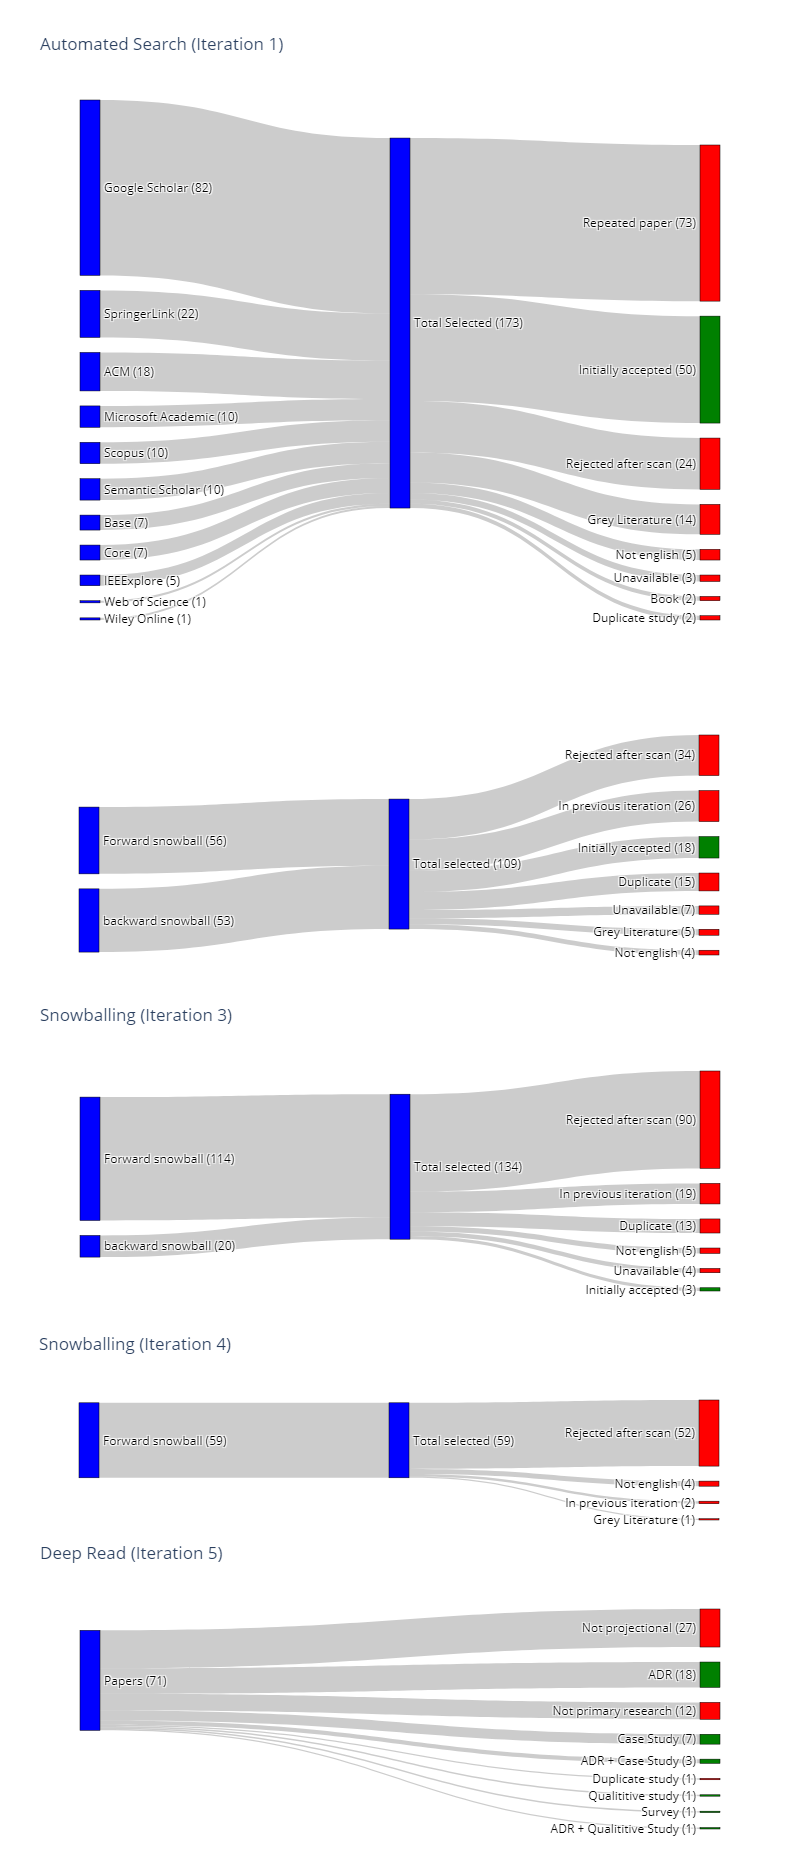
\includegraphics[width=0.75\textwidth]{/Sections/images/search_sankey.png}}
    \caption{Search results}
    \label{fig:search_results}
\end{figure}


Our final selection iteration involved a deeper scan of to determine of the remaining 71 papers.
With this we could reject 12 papers which were not primary research, one paper that reported a study already represented.
There were also 27 papers that were, on closer reading, not about projectional editing.

This left us with 31 papers before the quality assessment filter.

\subsubsection{sensitivity and precision}
As a curio, we reapproriated Zhang's\cite{Zhang_2011} ideas of sensitivity and precision and applied them to the search engines rather than search strings.
The values for sensitivity and precision of the search engines are calculated as follows:
\[
        sensitivity = \frac{\#\;retrieved\;relevant\;studies}{all\;relevant\;studies} \;100\%
\]

\[
        precision = \frac{\#\;retrieved\;relevant\;studies}{\#\;studies\;retrieved} \;100\%
\]

Table \ref{table:sensitivity_precision} show that Google Scholar had the highest sensitivity, returning 22 of the 31 chosen studies.
This came at the cost of a very large proportion of false positives.
Microsoft Academic and SpringerLink were joint most precise with half of their search results ending up in the final roster.
SpringerLink, with the second highest count of documents, second highest sensitivity, and joint highest precision would appear to be the best all around search engine for this field.
However, these figures are skewed by several of their articles coming from a single collection specifically about projectional editing.

\begin{table}[h]
    \begin{center}
        \begin{tabular}{ | l | c | c | c | c |} 
            \hline
            Search engine/library     & original \# & selected \# & sensitivity & precision\\
            \hline
            \hline
            ACM                        & 18          & 3           & 10\%        &  16\%    \\
            BASE                       & 7           & 3           & 10\%        &  43\%    \\
            CORE                       & 7           & 1           &  3\%        &  14\%    \\
            Google Scholar             & 82          & 22          & 71\%        &  27\%    \\
            IEEExplores                & 5           & 2           &  6\%        &  40\%    \\
            Microsoft Academic         & 10          & 5           & 16\%        &  50\%    \\
            Science.gov                & 0           & 0           &  0\%        &   0\%    \\
            SCOPUS                     & 10          & 3           & 10\%        &  30\%    \\
            Semantic Scholar           & 10          & 4           & 13\%        &  40\%    \\
            SpringerLink               & 22          & 11          & 35\%        &  50\%    \\
            Wiley Online               & 1           & 0           &  0\%        &   0\%    \\
            Web of Science             & 1           & 0           &  0\%        &   0\%    \\
            \hline
        \end{tabular}
    \end{center}
    \caption{Search Engine sensitivity and precision}
    \label{table:sensitivity_precision}
\end{table}


\subsection{Quality Assessment}
Using the quality assessment checklists, developed by Crombie et al.\cite{crombie1997pocket}, shown in Appendix \ref{appendix:QualityAssesmentChecklist} we examined the remaining 31 papers which on the surface represented 37 primary studies.
As Action Design Research was not represented amongst these checklists we searched for an appropriate quality assessment checklist for these type of primary study.
We did not find a suitable checklist, and did not consider ourselves suitably qualified to make one.
Thus we used the Case Study Quality Assessment Checklist to assess the ADR studies.

We used a rudimentary scoring system of +1 value for positive answers, 0 for ``don't knows'', and -1 for negative answers.
We arbitrarily chose that any study with an overall score greater than 0 would be considered high enough quality to be part of our final analysis.

With this scoring and goal we only found 6 out of 37 studies of high enough quality.

We therefore had to decide to change our scoring, go ahead with 6 studies, stop here or ignore the QA findings.
Changing the scoring until you get the ``right'' result felt wrong.
6 studies seems too few to give an overview of a field.
Stopping seems to be the correct course for an SLA.
However, we decided to create a new Quasi-SLA, that ignores the results of a Quality assessment.

Our reason to continue was that we could not reconcile that 84\% of studies that had made it to the recognized scientific journals were not of high enough quality to pass our SLR QA stage.
We believe there were two large threats to the validity of the Quality Assessment stage that were too great to ignore.
The first being that it was carried out by a single researcher with no previous experience.
The other being either that the use of Case Study Checklists is inappropriate for ADR studies or that ADR studies are inappropriate for SLRs.


\subsection{Analysis}
After Identifying the primary studies we extracted data, the details of which are shown in Appendix \ref{appendix:DataExtraction}.
A summary is shown in 
[TODO: lots of Graphs]

\subsection{Threats to validity}

\begin{itemize}
    \item survey selection
    \item quality assessment
    \item data extraction
    \item search phrase choice
    \item that sentiment analysis is invalid for scientific papers
    \item azure sentiment analysis is not calibrated for scientific papers
\end{itemize}
 